\documentclass{beamer}
\beamertemplatenavigationsymbolsempty
\usecolortheme{beaver}
\setbeamertemplate{blocks}[rounded=true, shadow=true]
\setbeamertemplate{footline}[page number]
%
\usepackage[utf8]{inputenc}
\usepackage[english,russian]{babel}
\usepackage{amssymb,amsfonts,amsmath,mathtext}
\usepackage{subfig}
\usepackage[all]{xy} % xy package for diagrams
\usepackage{array}
\usepackage{multicol}% many columns in slide
\usepackage{hyperref}% urls
\usepackage{hhline}%tables
% Your figures are here:
\graphicspath{ {fig/} {../fig/} }

%----------------------------------------------------------------------------------------------------------
\title[\hbox to 56mm{Порождающие модели для прогнозирования}]{Порождающие модели для прогнозирования (наборов временных рядов) в метрическом вероятностном пространстве}
\author[Г.\,А. Карпеев]{Карпеев Глеб Андреевич}
\institute{Московский физико-технический институт}
\date{\footnotesize
\par\smallskip\emph{Курс:} Автоматизация научных исследований\par (практика, В.\,В.~Стрижов)/Группа 128
\par\smallskip\emph{Эксперт:} В.\,В.~Стрижов
\par\smallskip\emph{Консультант:} К.~Яковлев
\par\bigskip\small 2024}
%----------------------------------------------------------------------------------------------------------
\begin{document}
%----------------------------------------------------------------------------------------------------------
\begin{frame}
\thispagestyle{empty}
\maketitle
\end{frame}
%-----------------------------------------------------------------------------------------------------
% \begin{frame}{Порождающие модели для прогнозирования наборов временных рядов}
% %\begin{block}{Решается задача}
% %\end{block}
% \end{frame}
%-----------------------------------------------------------------------------------------------------
\begin{frame}{Порождающие модели для прогнозирования наборов временных рядов}

% Пожалуйста, уберите прочие слайды, если у вас доклад с одним слайдом.

\begin{columns}[c]
\column{0.5\textwidth}

\begin{columns}[c]
\column{0.5\textwidth}
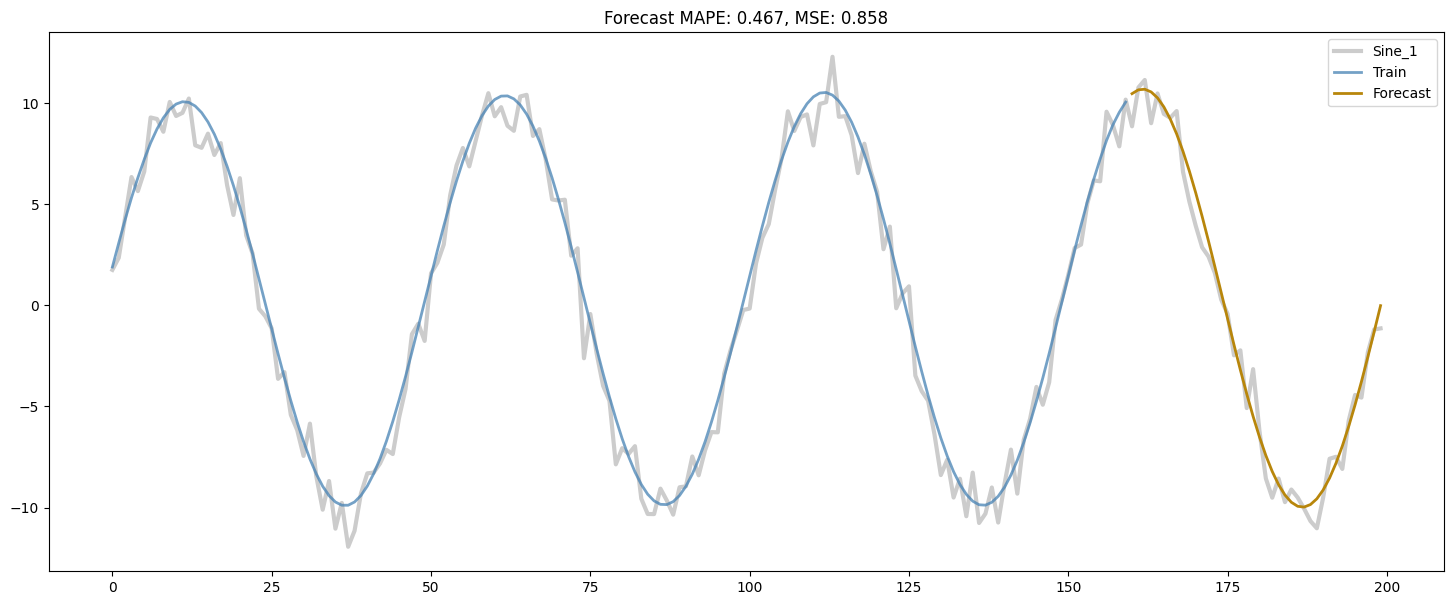
\includegraphics[width=1\textwidth]{fig/sin_mssa_small_ampl.png}
\column{0.5\textwidth}
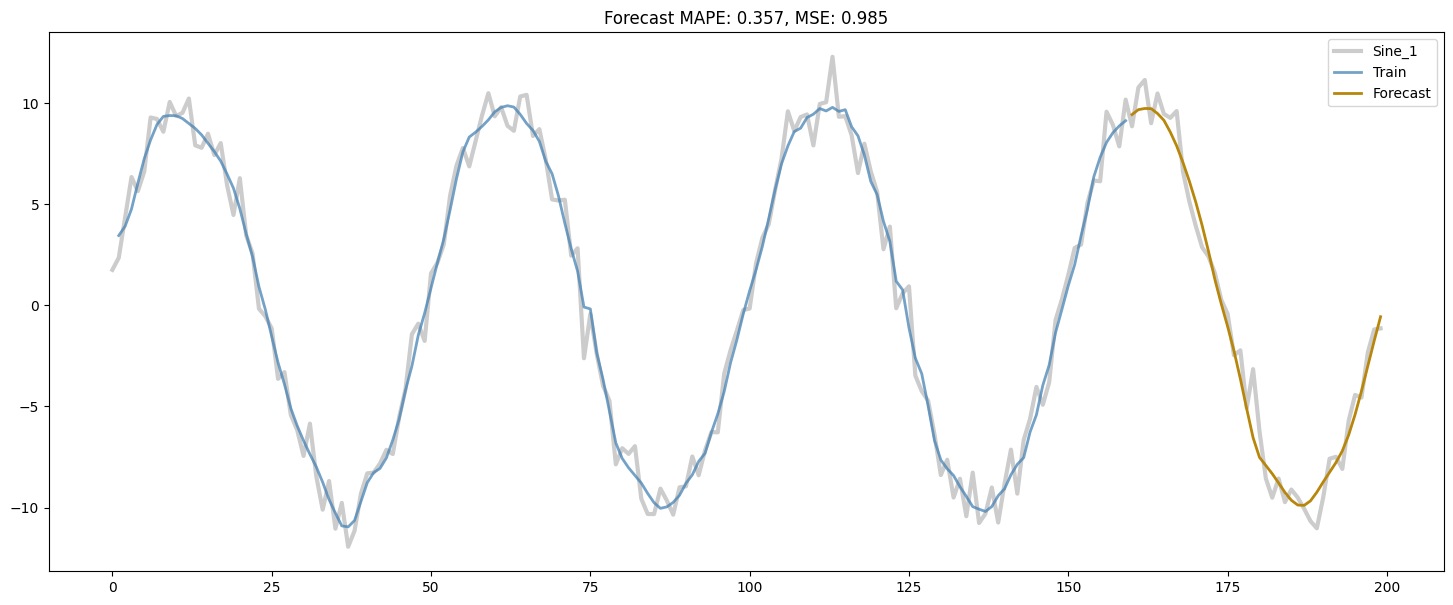
\includegraphics[width=1\textwidth]{fig/sin_lstm_small_ampl.png}
\end{columns}
    Прогноз синтетических данных с небольшим шумом с помощью MSSA и LSTM

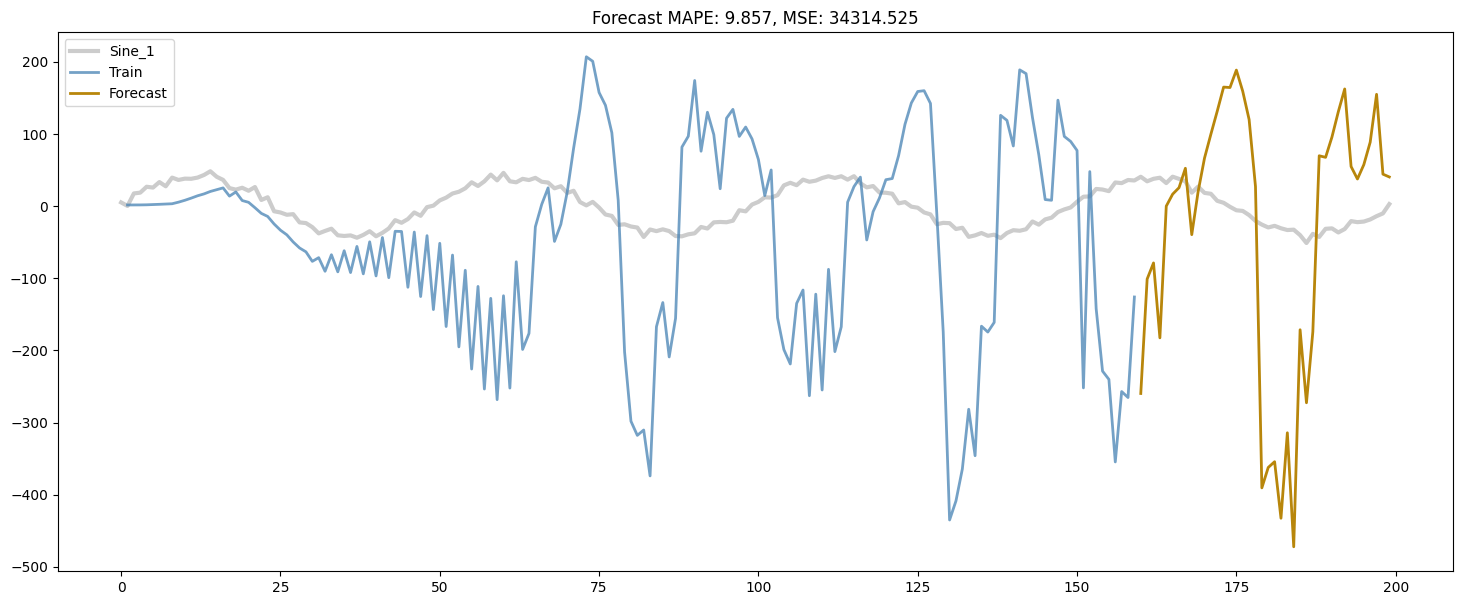
\includegraphics[width=1\textwidth]{fig/sin_lstm_high_ampl.png}
    Прогноз синтетических данных с большим шумом с помощью LSTM
\column{0.5\textwidth}
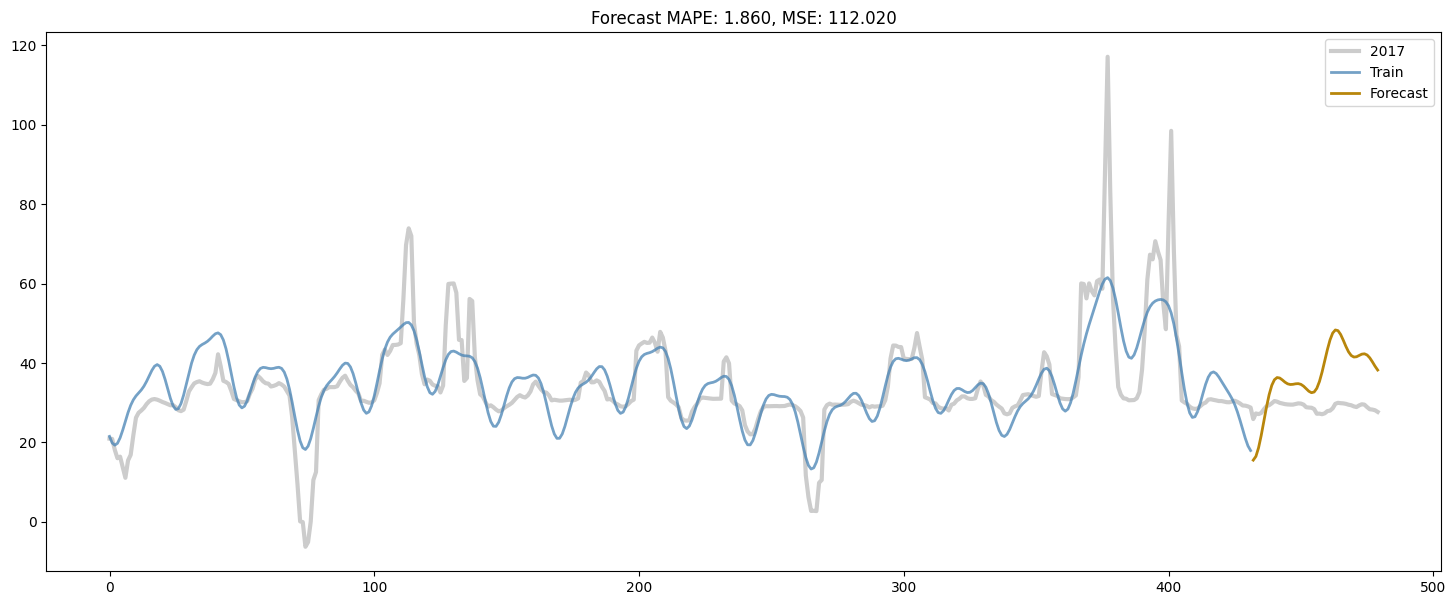
\includegraphics[width=1.0\textwidth]{real_data_2017.png}
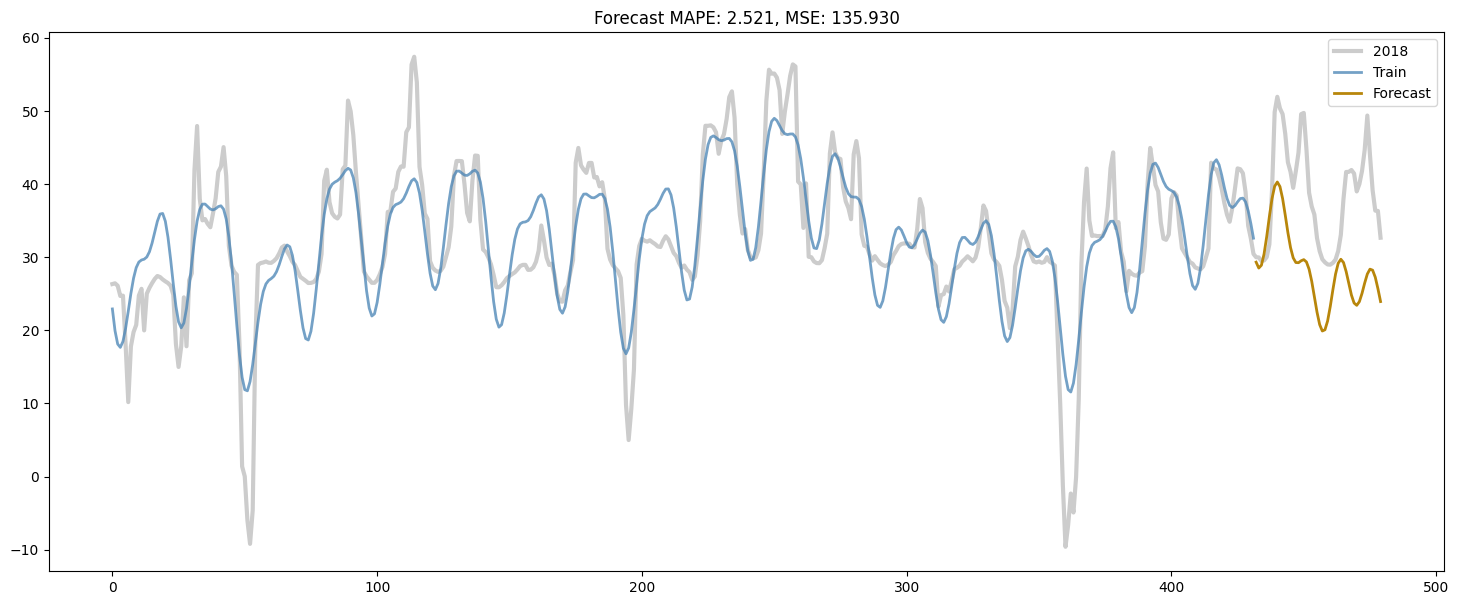
\includegraphics[width=1.0\textwidth]{real_data_2018.png}
    Прогноз спотовых цен на электроэнергию методом MSSA
\end{columns}

% \bigskip
% Важное {\color{red}сообщение}.
\end{frame}


%----------------------------------------------------------------------------------------------------------
% \begin{frame}{Постановка задачи}

% \end{frame}
%----------------------------------------------------------------------------------------------------------
% \begin{frame}{Решение}
% \begin{columns}[c]
% \column{0.6\textwidth}
%     Столбец 1
% \column{0.4\textwidth}
%     Столбец 2
% \end{columns}
% \end{frame}
%----------------------------------------------------------------------------------------------------------
% \begin{frame}{Вычислительный эксперимент}

%  Что зритель видит на графике.

% \includegraphics[width=0.8\textwidth]{ErrorFunction}

% О чем говорит этот график.

% \end{frame}
%----------------------------------------------------------------------------------------------------------
% \begin{frame}{Заключение}
%     \begin{block}{Перечислите ваши результаты}
%     \begin{itemize}
%         \item предложен метод,
%         \item доказана теорема.
%     \end{itemize}
%     \end{block}
% \end{frame}
%----------------------------------------------------------------------------------------------------------
\end{document} 